\documentclass[10pt]{article}
\usepackage[margin=0.8in]{geometry}
\usepackage{graphicx,booktabs,amsmath}
\usepackage[font=small]{caption}
\setlength{\parskip}{3pt}\setlength{\parindent}{0pt}
\begin{document}
\begin{center}{\large\bf The 15:30 forecast's weights, and when sign(s) makes money}\\[2pt]
{\small 866 deck days, 2020-01-03 .. 2024-04-30; forecast of record: per-bar ridge, live-feasible features, 2000-session window, bar ending 16:00}\end{center}

\textbf{Question.} Which inputs move the 15:30 variance forecast, how stable are their weights, and do the weights or the inputs' contributions line up with the days on which sign(s) (buy the nearest-OTM 0DTE package if $s=\hat{rv}-iv>0$, sell otherwise, settle at the close) makes money?

\textbf{Verification (before any reading).} The fitted coefficients are not stored, so the forecast was re-run with the research code and the coefficient vector recorded at every refit.
(1) The re-run equals the stored forecast on all 1,469 rows of the 16:00 bar (max relative difference $7.3\times10^{-12}$).
(2) Coefficients $\cdot$ inputs $+$ intercept reproduce every forecast to $2.1\times10^{-15}$, and forecast $=$ level $+\sum_j$ contribution$_j$ to $1.2\times10^{-15}$, where contribution$_j=\beta_j(x_j-\bar x_j)$ over the trailing window and the level is the window-mean target (to $4.9\times10^{-13}$).
(3) All 866 deck days join (bar-end 16:00 ET row $=$ forecast issued at 15:30); 52 are month-end sessions.
Standardized weight $=\beta_j\times$ trailing-window sd of $x_j$. Intervals: circular block bootstrap, block $\lceil n^{1/3}\rceil$, 2,000 draws; $^{*}$ = 95\% interval excludes 0.

\textbf{Money on this forecast.} Summed return per premium: mid $+102.98$ (month-ends $-10.67$, other days $+113.65$); crossed (buy at the ask, sell at the bid) $+74.15$ ($-12.94$ / $+87.09$). It buys 348 of 866 days and only 10 of the 52 month-ends.

\begin{figure}[h]\centering
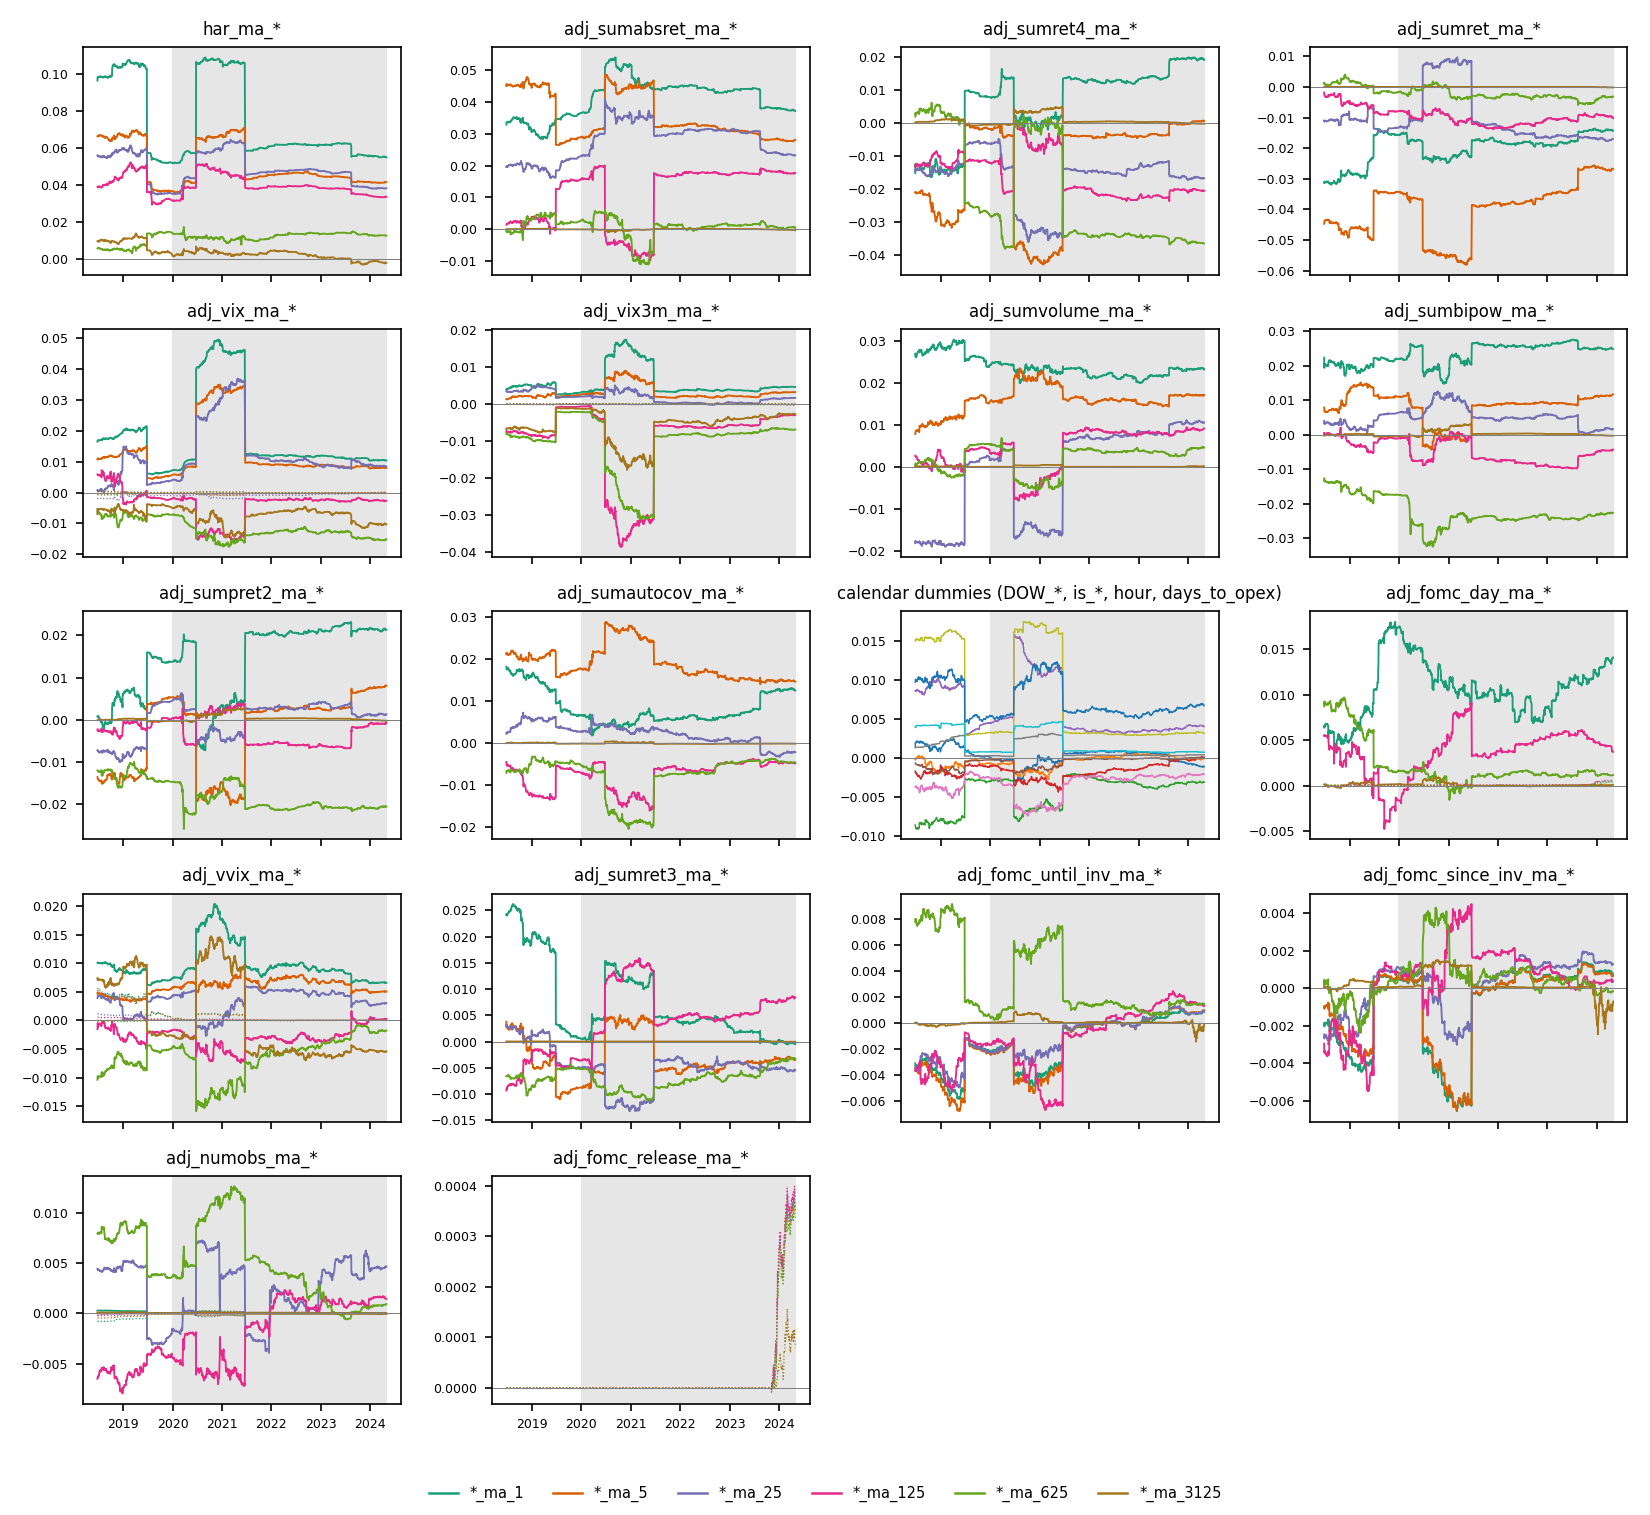
\includegraphics[width=\textwidth]{../results/model_diagnostics_1530/weights_small_multiples.png}
\caption{Standardized weights over every refit (1,469 sessions), one panel per input series; solid = the series' rolling means (colour = window length in 30-minute bars). Panel titles are the design's column names; \texttt{*\_ma\_$k$} is the mean over the last $k$ 30-minute bars (\texttt{\_ma\_1} = the last bar), \texttt{adj\_} marks the series after its transform (e.g. log for the VIX) and diurnal adjustment, and the dotted lines are the \texttt{*\_avail\_ma\_$k$} / \texttt{*\_active\_ma\_$k$} is-present / is-nonzero flags. Key: \texttt{har\_ma} realized variance (the target); \texttt{sumret} signed return; \texttt{sumabsret} absolute return; \texttt{sumret3} cubed returns (skew); \texttt{sumret4} 4th-power returns (tails); \texttt{sumpret2} upside squared returns; \texttt{sumbipow} bipower variation; \texttt{sumautocov} return autocovariance; \texttt{sumvolume} ES volume (contracts); \texttt{numobs} ES trade count per bar; \texttt{vix}, \texttt{vvix}, \texttt{vix3m} the Cboe indices; \texttt{fomc\_release} FOMC statement bar; \texttt{fomc\_day} FOMC day; \texttt{fomc\_until\_inv} / \texttt{fomc\_since\_inv} 1 / days to the next / since the last FOMC. Grey band = the 866 deck days. 138 of the 244 design columns carry a nonzero weight on deck days; the rest are constant or duplicated within the window and are masked to zero.}
\end{figure}

\begin{table}[h]\centering\small
\caption{The 12 inputs that move the forecast most on the deck days (by sd of their contribution; forecast sd 0.357 in the same units).}
\begin{tabular}{lrrrr}\toprule
input & mean std.\ weight & sd & days $>0$ & contribution sd\\\midrule
realized variance (target), last bar & +0.068 & 0.018 & 100\% & 0.066 \\
4th-power returns (tails), mean of last 625 bars & -0.028 & 0.013 & 6\% & 0.045 \\
realized variance (target), mean of last 5 bars & +0.048 & 0.009 & 100\% & 0.044 \\
realized variance (target), mean of last 25 bars & +0.047 & 0.007 & 100\% & 0.041 \\
absolute return, last bar & +0.043 & 0.004 & 100\% & 0.040 \\
signed return, mean of last 5 bars & -0.038 & 0.009 & 0\% & 0.040 \\
bipower variation, mean of last 625 bars & -0.024 & 0.002 & 0\% & 0.035 \\
realized variance (target), mean of last 125 bars & +0.039 & 0.005 & 100\% & 0.033 \\
absolute return, mean of last 5 bars & +0.033 & 0.006 & 100\% & 0.032 \\
upside squared returns, mean of last 625 bars & -0.020 & 0.002 & 0\% & 0.031 \\
absolute return, mean of last 25 bars & +0.030 & 0.004 & 100\% & 0.029 \\
VIX, last bar & +0.017 & 0.013 & 100\% & 0.027 \\
\bottomrule\end{tabular}\end{table}

\begin{figure}[h]\centering
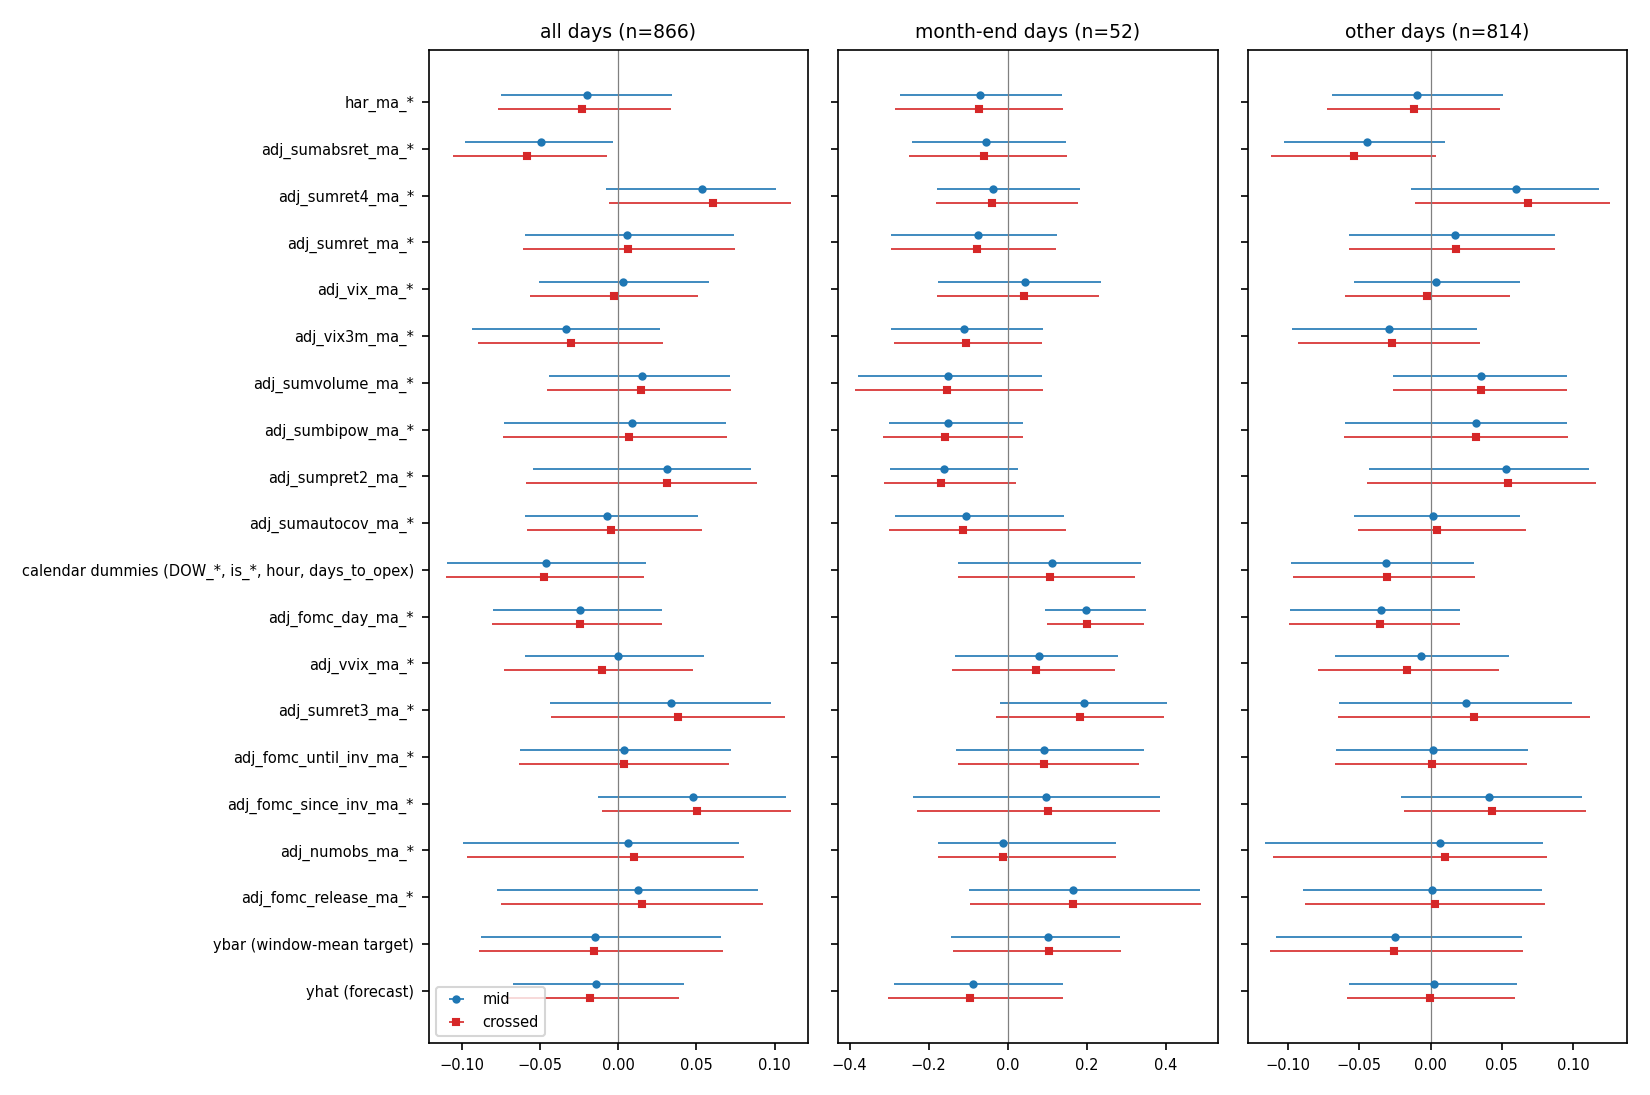
\includegraphics[width=\textwidth]{../results/model_diagnostics_1530/corr_contribution_vs_pnl.png}
\caption{Correlation across deck days of each input series' summed contribution (rows named by the design's columns, key under Figure 1; \texttt{ybar} = the level, \texttt{yhat} = the forecast) to the forecast with the day's return per premium (blue mid, red crossed), 95\% block-bootstrap intervals.}
\end{figure}

\begin{table}[h]\centering\small
\caption{Series contribution vs the day's return per premium (the top 8 series by contribution sd, the FOMC-day flag, and the forecast itself).}
\begin{tabular}{lrrrrrr}\toprule
 & \multicolumn{2}{c}{all (866)} & \multicolumn{2}{c}{month-ends (52)} & \multicolumn{2}{c}{other (814)}\\
series & mid & crossed & mid & crossed & mid & crossed\\\midrule
realized variance (target) & -0.02 & -0.02 & -0.07 & -0.07 & -0.01 & -0.01 \\
absolute return & -0.05$^{*}$ & -0.06$^{*}$ & -0.06 & -0.06 & -0.04 & -0.05 \\
4th-power returns (tails) & +0.05 & +0.06 & -0.04 & -0.04 & +0.06 & +0.07 \\
signed return & +0.01 & +0.01 & -0.08 & -0.08 & +0.02 & +0.02 \\
VIX & +0.00 & -0.00 & +0.04 & +0.04 & +0.00 & -0.00 \\
VIX3M & -0.03 & -0.03 & -0.11 & -0.11 & -0.03 & -0.03 \\
ES volume & +0.02 & +0.01 & -0.15 & -0.15 & +0.04 & +0.04 \\
bipower variation & +0.01 & +0.01 & -0.15 & -0.16 & +0.03 & +0.03 \\
FOMC day flag & -0.02 & -0.02 & +0.20$^{*}$ & +0.20$^{*}$ & -0.03 & -0.04 \\
forecast (sum) & -0.01 & -0.02 & -0.09 & -0.10 & +0.00 & -0.00 \\
\bottomrule\end{tabular}

\vspace{4pt}
Feature level (138 inputs): intervals excluding 0, standardized weight / contribution (chance $\approx$ 7 of 138)\\[2pt]
\begin{tabular}{lccc}\toprule
split & mid P\&L & crossed P\&L & buy decision\\\midrule
all & 1 / 14 & 0 / 16 & 37 / 21 \\
month-end & 4 / 13 & 4 / 16 & 1 / 7 \\
other & 0 / 5 & 0 / 7 & 38 / 27 \\
\bottomrule\end{tabular}\end{table}

\begin{figure}[h]\centering
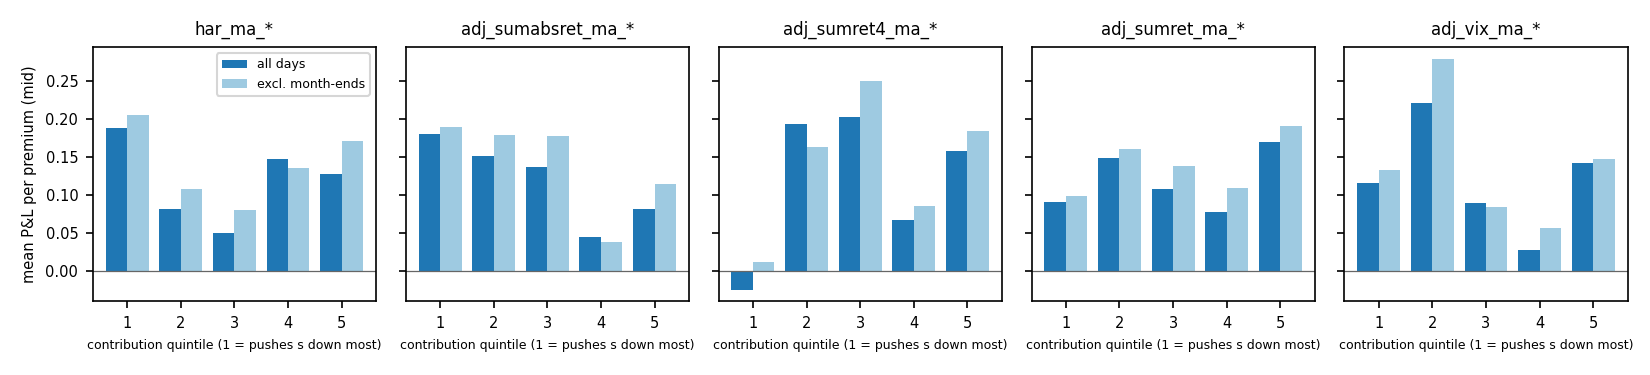
\includegraphics[width=\textwidth]{../results/model_diagnostics_1530/pnl_by_contribution_quintile.png}
\caption{Mean mid return per premium by quintile of each of the five largest series' contributions (named by the design's columns, key under Figure 1) (dark: all 866 days; light: without month-ends).}
\end{figure}

\begin{table}[h]\centering\small
\caption{What drives the decision: correlation of the two sides of $s$ with the day's mid return and with the buy decision ($+1$ buy, $-1$ sell). $\log\hat{rv}$ = log diurnal scale (not a regression output) $+$ the regression part.}
\begin{tabular}{lrrrrrr}\toprule
 & \multicolumn{2}{c}{all} & \multicolumn{2}{c}{month-ends} & \multicolumn{2}{c}{other}\\
 & mid & decision & mid & decision & mid & decision\\\midrule
log forecast $\hat{rv}$ & -0.05 & -0.02 & -0.02 & +0.03 & -0.05 & -0.02 \\
log implied variance & -0.06 & -0.25$^{*}$ & -0.07 & -0.20 & -0.05 & -0.25$^{*}$ \\
$\log(\hat{rv}/iv)$ (sign = decision) & +0.04 & +0.76$^{*}$ & +0.17 & +0.70$^{*}$ & +0.02 & +0.76$^{*}$ \\
log diurnal scale of $\hat{rv}$ & -0.05 & -0.05 & +0.02 & +0.13 & -0.06 & -0.06 \\
regression part of $\log\hat{rv}$ & -0.00 & +0.04 & -0.05 & -0.13 & +0.01 & +0.06 \\
log diurnal scale $-$ log implied & +0.02 & +0.33$^{*}$ & +0.12 & +0.43$^{*}$ & -0.00 & +0.31$^{*}$ \\
\bottomrule\end{tabular}\end{table}

\textbf{Reading.}
\begin{itemize}\itemsep1pt
\item \emph{The weights keep their sign and move in steps.} The penalty is re-chosen every 250 refits (1000, the top of the grid, on 712 of 866 deck days; 100 on the rest), and the inputs that move the forecast most keep one sign on every deck day: realized variance in the last bar ($+0.068$, sd 0.018), its 5- and 25-bar means ($+0.048$, $+0.047$), absolute return in the last bar ($+0.043$), the 5-bar signed return ($-0.038$). The forecast is a HAR on realized variance and absolute returns (series contribution sd 0.170 and 0.111), trimmed by long-window tail, bipower and upside terms (negative weights), with VIX adding and VIX3M subtracting (0.038 / 0.037).
\item \emph{Weights do not track money.} Across 138 inputs, 1 standardized-weight interval excludes zero for the mid return on all days (0 crossed; 0 on non-month-end days) -- below the $\approx$7 expected by chance. They do co-move with the buy/sell mix (37 of 138 exclude zero for the decision): both drift slowly over the sample, which is not a day-level link to the return.
\item \emph{Contributions barely track money.} 14 (mid) and 16 (crossed) of 138 contribution intervals exclude zero on all days, against $\approx$7 by chance; on non-month-end days 5 and 7, i.e.\ chance. At the series level only absolute return is outside zero on all days ($-0.049$ mid, $-0.058$ crossed): days on which recent absolute returns push the forecast up earn less. The forecast itself: $-0.014$ [$-0.07$, $+0.04$]. No quintile pattern is monotone (Figure 3).
\item \emph{The decision is set by the implied side and the diurnal scale, not by the weights.} $\log(\hat{rv}/iv)$ has variance 0.101 while each side has about 1 (correlation 0.952); of $\log\hat{rv}$'s variance 0.967, the diurnal scale carries 0.813 and the regression part 0.365 (covariance $-0.211$). The regression part correlates $+0.04$ with the decision (interval through zero); log implied variance $-0.25$ on non-month-end days. Of the 330 day-to-day decision changes, the forecast moved more than the implied on 134.
\item \emph{Month-ends.} This forecast sells 42 of the 52 month-ends and loses there. On month-ends the FOMC-day flag's contribution correlates $+0.20$ with the day's return (interval $+0.09$ .. $+0.35$); on the 10 month-end buys (4 winners, 6 losers) the winners had lower absolute-return and ES-volume contributions and higher tail contributions. Both rest on a handful of days.
\end{itemize}
Files: \texttt{experiments/model\_diagnostics\_1530.py} (capture, then analyze); outputs in \texttt{results/model\_diagnostics\_1530/}.

\clearpage
\begin{center}{\large\bf Regime changes, which inputs dominate, and how the lasso picks out the VIX}\\[2pt]
{\small same forecast, same 16:00 bar; 1,469 refits (2018-06-25 .. 2024-04-30), of which 866 are deck days}\end{center}

\textbf{1. Regime changes.} \emph{Question:} do the weights, and the trade's money, change at the known dates -- the penalty switches (2019-06-26, 2020-06-23, 2021-06-21), the Feb--Apr 2020 crash (2020-02-20 .. 2020-04-30, from the session after the S\&P high on the deck, 2020-02-19), the start of every-day expirations -- and is a change the penalty or the data?

\emph{Gate.} Two more re-runs of the same arm with the penalty held at one value: held at 100 it equals the arm of record on all 500 refits where the record used 100 (to $2.6\times10^{-12}$), held at 1000 on all 969 refits at 1000 (to $9.6\times10^{-14}$). The arm of record is the two held-penalty runs spliced at the switch dates, so a change that neither held run shows is the penalty.
\emph{Every-day expirations.} The first Tuesday/Thursday deck day is 2020-01-21 (a holiday-shifted expiry); every Tuesday session is a deck day from 2022-04-26 and every Thursday from 2022-05-19; the tests use 2022-04-26.
\emph{Tests.} Known date: Chow test in Wald form with Newey--West covariance (lag $\lfloor 4(n/100)^{2/9}\rfloor$ = 7 on refits, 6 on deck days), $\chi^2(p)$, run only where each side holds at least 15\% of the sample; the Feb--Apr 2020 episode (50 refits, 32 deck days) by Chow's predictive $F$ test, the standard test for a stretch too short to fit on its own. Unknown date: Andrews' sup-Wald over the middle 70\% of the sample, critical values simulated from its limit (20,000 draws; $p=1$, 5\%: 8.73, published 8.58--8.85). Regressions: the 16:00 target on the forecast (calibration, $p=2$); the target on the contributions of the six largest series plus the rest summed ($p=8$); the day's return per premium on a constant ($p=1$), and on the same contributions ($p=8$).

\begin{figure}[h]\centering
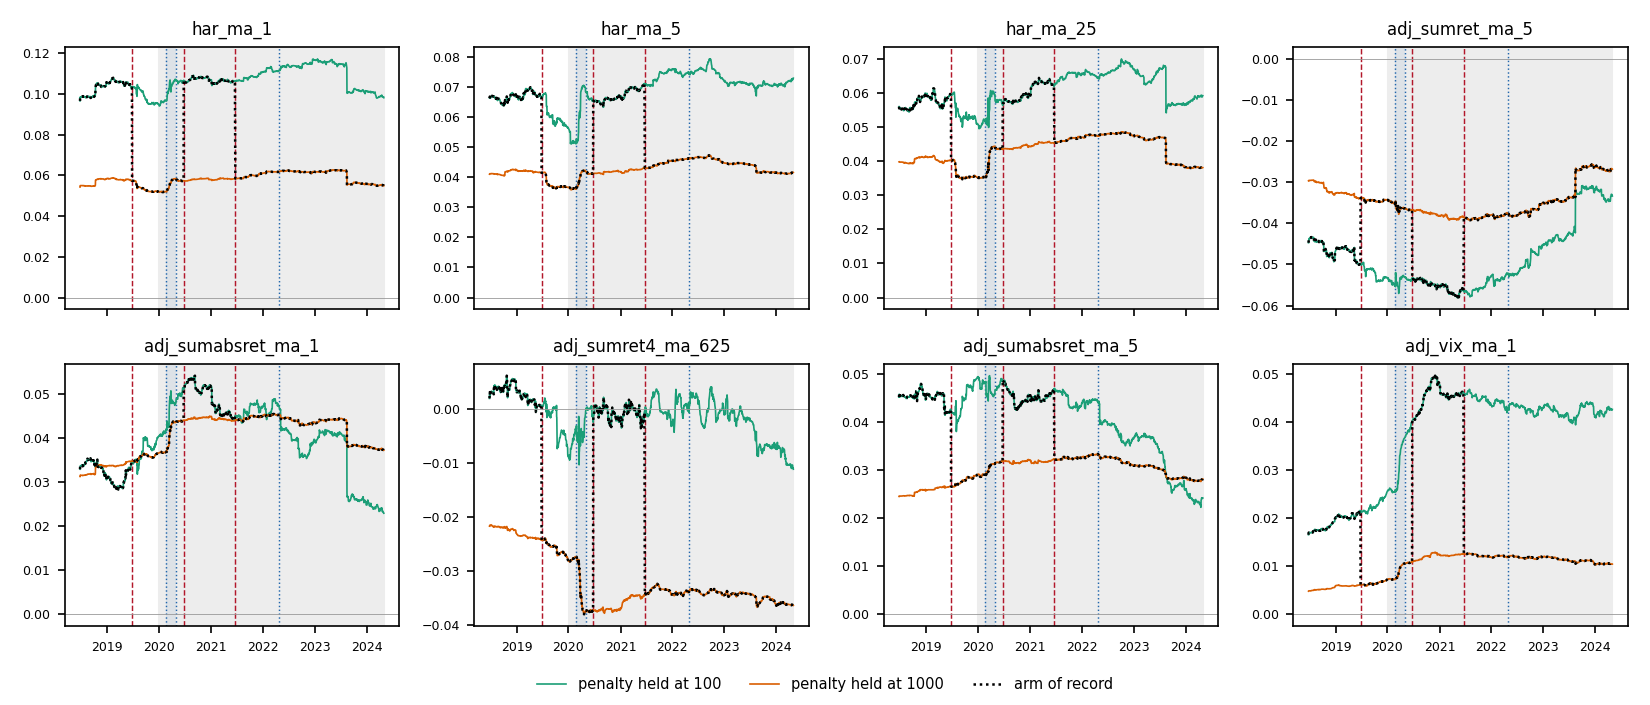
\includegraphics[width=\textwidth]{../results/model_diagnostics_1530/regimes_weights_counterfactual.png}
\caption{Standardized weights of the eight largest inputs (design column names, key under Figure 1): the arm of record (dotted black) and the same arm with the penalty held at 100 (green) or 1000 (orange). Red dashed = penalty switches; blue dotted = COVID start/end and every-day expirations; blue band = Feb--Apr 2020; grey = deck days.}
\end{figure}

\begin{table}[h]\centering\small
\caption{The step in all standardized weights at each penalty switch (Euclidean norm across inputs), split into the penalty (the two held runs on the same day) and one more day of data (the old penalty's run, day over day).}
\begin{tabular}{llrrrrr}\toprule
date & penalty & step & penalty part & data part & largest step, other days & median \\\midrule
2019-06-26 & 100 to 1000 & 0.0932 & 0.0930 & 0.0010 & 0.0199 & 0.00062 \\
2020-06-23 & 1000 to 100 & 0.1177 & 0.1177 & 0.0008 & 0.0199 & 0.00062 \\
2021-06-21 & 100 to 1000 & 0.1232 & 0.1235 & 0.0022 & 0.0199 & 0.00062 \\
\bottomrule\end{tabular}\end{table}

\begin{table}[h]\centering\scriptsize
\caption{Break tests: $p$-values at the known dates and for the COVID episode, and the unknown-date sup-Wald (statistic, date of its maximum, $p$). record = the arm of record; 100 / 1000 = penalty held. -- = not testable (before the deck, or under 15\% of the deck days on one side). $^{*}$ = $p<0.05$; with seven dates per row, a stray $^{*}$ is expected by chance.}
\setlength{\tabcolsep}{2.5pt}
\resizebox{\textwidth}{!}{\begin{tabular}{llrrrrrrrrl}\toprule
regression & pen. & $p$ & pen. 100 to 1000 & COVID start & COVID end & pen. 1000 to 100 & pen. 100 to 1000 & every-day & COVID & sup-Wald \\
 & & & 2019-06-26 & 2020-02-20 & 2020-05-01 & 2020-06-23 & 2021-06-21 & 2022-04-26 & episode & \\\midrule
target on forecast & record & 2 & 0.713 & 0.867 & 0.191 & 0.119 & 0.034$^{*}$ & 0.040$^{*}$ & $<$0.001$^{*}$ & 7.4 (2021-06-02) 0.262 \\
 & 100 & 2 & 0.672 & 0.724 & 0.623 & 0.435 & 0.599 & 0.589 & $<$0.001$^{*}$ & 2.6 (2020-09-29) 0.931 \\
 & 1000 & 2 & 0.727 & 0.975 & 0.194 & 0.105 & 0.210 & 0.204 & $<$0.001$^{*}$ & 5.4 (2020-07-14) 0.515 \\
\midrule
target on contributions & record & 8 & 0.002$^{*}$ & 0.159 & 0.119 & 0.047$^{*}$ & 0.232 & 0.022$^{*}$ & $<$0.001$^{*}$ & 29.1 (2022-10-11) 0.007$^{*}$ \\
 & 100 & 8 & 0.023$^{*}$ & 0.181 & 0.103 & 0.149 & 0.190 & 0.280 & $<$0.001$^{*}$ & 28.9 (2020-04-09) 0.008$^{*}$ \\
 & 1000 & 8 & 0.464 & 0.648 & 0.006$^{*}$ & 0.021$^{*}$ & 0.076 & 0.008$^{*}$ & $<$0.001$^{*}$ & 40.0 (2022-10-11) $<$0.001$^{*}$ \\
\midrule
mean return, mid & record & 1 & -- & -- & -- & -- & 0.791 & 0.779 & 0.768 & 2.2 (2023-01-04) 0.752 \\
mean return, crossed & record & 1 & -- & -- & -- & -- & 0.962 & 0.569 & 0.679 & 2.8 (2023-01-04) 0.615 \\
\midrule
return on contributions & record & 8 & -- & -- & -- & -- & 0.011$^{*}$ & 0.003$^{*}$ & 0.600 & 25.4 (2021-06-09) 0.028$^{*}$ \\
 & 1000 & 8 & -- & -- & -- & -- & 0.007$^{*}$ & 0.004$^{*}$ & 0.537 & 27.0 (2021-02-12) 0.017$^{*}$ \\
\bottomrule\end{tabular}}\end{table}

\begin{figure}[h]\centering
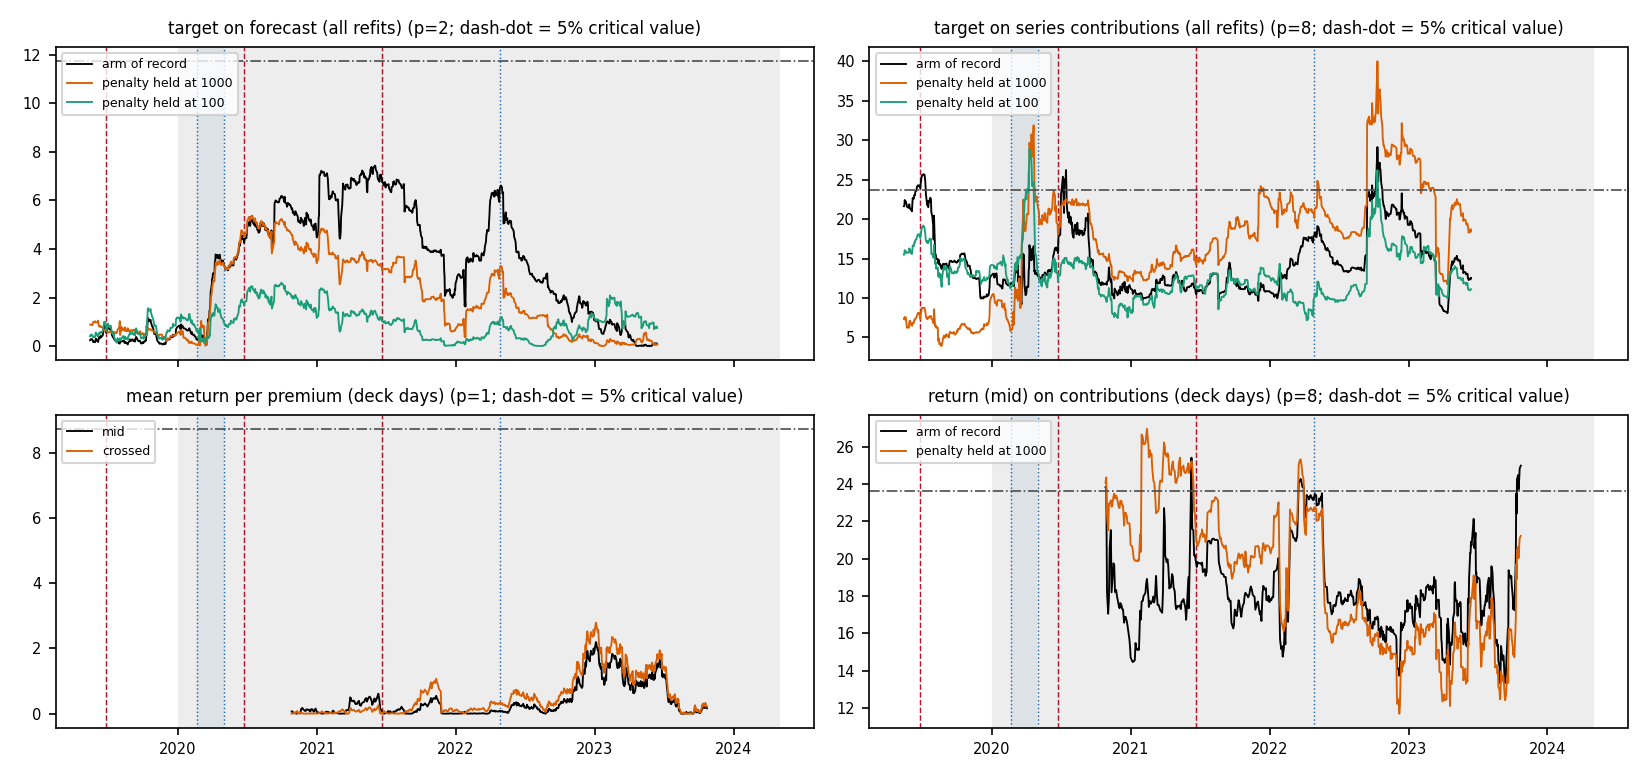
\includegraphics[width=\textwidth]{../results/model_diagnostics_1530/regimes_supwald_paths.png}
\caption{Wald statistic for a break at each date (the sup-Wald scan) with its 5\% critical value. Vertical lines as in Figure 4.}
\end{figure}

\textbf{Reading.}
\begin{itemize}\itemsep1pt
\item \emph{Every step in the weights is the penalty.} At the three switches all weights together jump by 0.093, 0.118, 0.123, of which the penalty is 0.093, 0.118, 0.123; on every other refit the largest step is 0.020 and the median 0.0006. Held at one penalty the weights drift smoothly through COVID and through every-day expirations (Figure 4).
\item \emph{The forecast's calibration does not break.} Target on forecast: sup-Wald 7.43 ($p$ 0.26); held at 100 / 1000: 2.61 / 5.37. The two known-date rejections in the arm of record (2021-06-21, $p$ 0.034; 2022-04-26, $p$ 0.040) vanish with the penalty held ($p\ge$ 0.20): made by the penalty. The Feb--Apr 2020 episode rejects under every penalty ($p<0.001$); the predictive test reacts to the crash's larger misses as well as to a changed slope.
\item \emph{How the series' contributions map into realized variance does change, and not because of the penalty.} The sup-Wald rejects under each penalty (29.1, 28.9, 40.0; $p\le$ 0.008), its maximum at 2022-10-11 (record, held 1000) or 2020-04-09 (held 100): one date is not pinned down. The COVID episode differs under every penalty. At the known dates the answer depends on which penalty is held (e.g. 2022-04-26: record 0.022, held 100 0.28, held 1000 0.008), so none is a clean data break.
\item \emph{The trade's money has no break in level.} Mean return per premium: sup-Wald 2.19 mid / 2.79 crossed ($p$ 0.75 / 0.61); the COVID days' mean is not different ($p$ 0.77 / 0.68). The return's slopes on the contributions do shift (sup-Wald 25.4, $p$ 0.028, at 2021-06-09; held 1000: 27.0, $p$ 0.017) -- the data, not the penalty -- but these are eight slopes on heavy-tailed returns that are near zero on either side (Table 2).
\item \emph{Not testable on the money:} 2019-06-26 is before the deck; the COVID start/end and 2020-06-23 leave under 15\% of the deck days on one side.
\end{itemize}

\clearpage
\textbf{2. Which series dominate (rolling SHAP).} \emph{Question:} which input series carry the forecast, and does that change across regimes?

\emph{Why the contributions are the SHAP values.} For a linear forecast $\hat y=\beta_0+\sum_j\beta_j x_j$ with the window mean $\bar x$ as the baseline (interventional SHAP), the SHAP value of input $j$ is exactly $\beta_j(x_j-\bar x_j)$, and the values sum to $\hat y$ minus the forecast at $\bar x$. \emph{Gate.} The \texttt{shap} library's LinearExplainer (the window mean as its one background row) on 8 refits (the first, the last, and each candidate date) equals $\beta_j(x_j-\bar x_j)$ to $0$, and its values plus the baseline equal the forecast to $1.6\times10^{-16}$ (relative). A series' SHAP value is the sum over its columns (all lags and flags). Share = the series' mean $|$SHAP$|$ over a trailing window divided by the sum over series. The window is a choice: 63 sessions (a quarter), checked against 126 (a half-year).

\begin{figure}[h]\centering
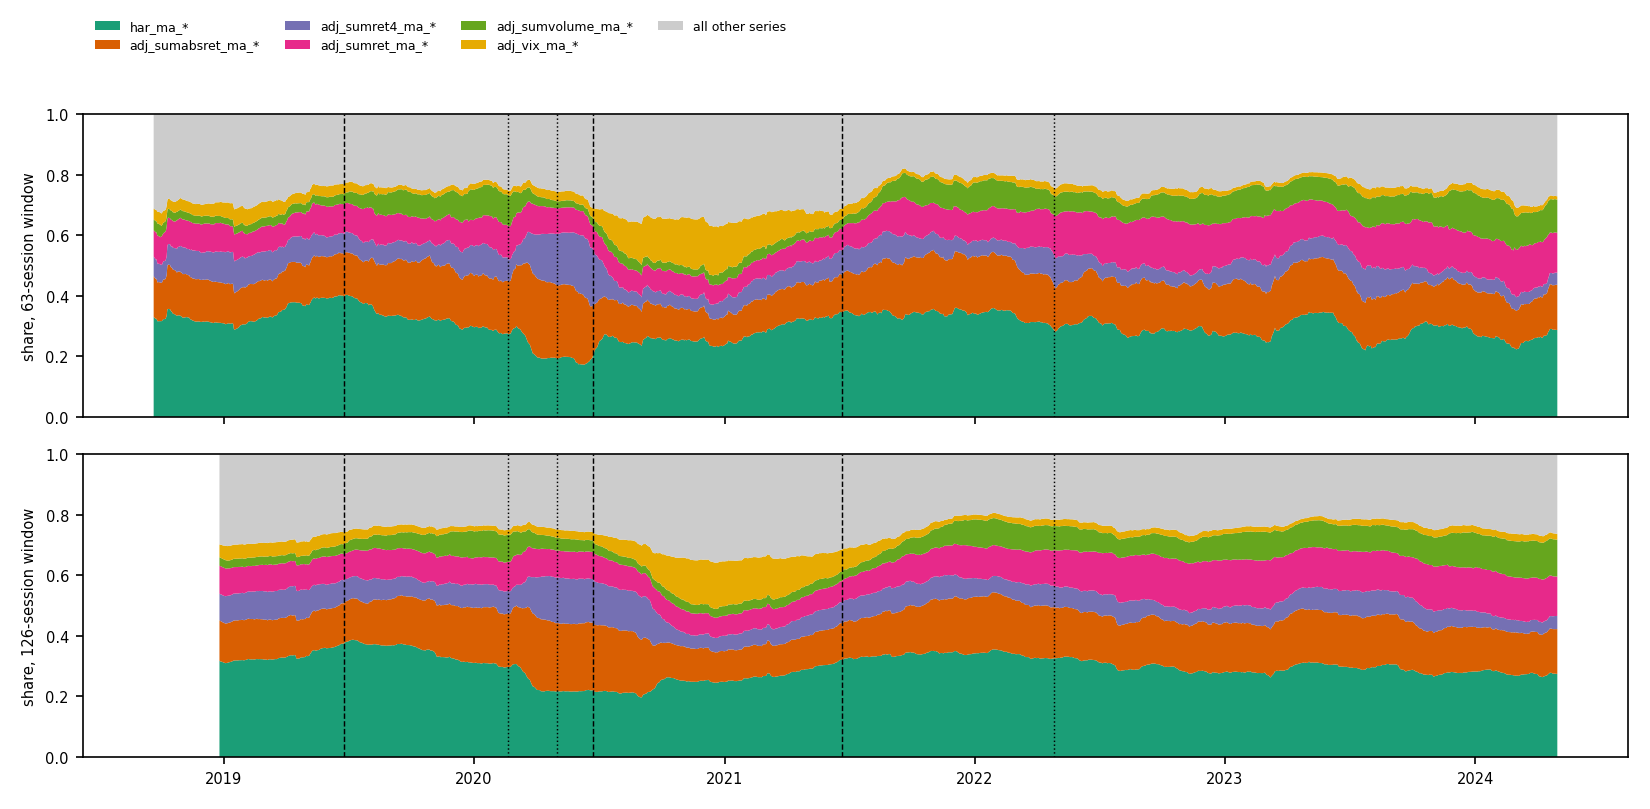
\includegraphics[width=\textwidth]{../results/model_diagnostics_1530/regimes_shap_share.png}
\caption{Share of mean $|$SHAP$|$ by input series (design column names, key under Figure 1), trailing 63 sessions (top) and 126 sessions (bottom). Dashed = penalty switches; dotted = COVID start/end and every-day expirations.}
\end{figure}

\begin{table}[h]\centering\scriptsize
\caption{The three largest series by share of mean $|$SHAP$|$ within each regime (cut at the candidate dates; no rolling), and the second and third with the penalty held at 1000.}
\resizebox{\textwidth}{!}{\begin{tabular}{lrrlllll}\toprule
regime & refits & deck days & penalty & first & second & third & held 1000: second / third \\\midrule
2018-06-25 .. 2019-06-25 & 250 & 0 & 100 & \texttt{har\_ma\_*} 35\% & \texttt{adj\_sumabsret\_ma\_*} 13\% & \texttt{adj\_sumret\_ma\_*} 9\% & \texttt{adj\_sumabsret\_ma\_*} / \texttt{adj\_sumret\_ma\_*} \\
2019-06-26 .. 2020-02-19 & 164 & 21 & 1000 & \texttt{har\_ma\_*} 30\% & \texttt{adj\_sumabsret\_ma\_*} 18\% & \texttt{adj\_sumret\_ma\_*} 10\% & \texttt{adj\_sumabsret\_ma\_*} / \texttt{adj\_sumret\_ma\_*} \\
2020-02-20 .. 2020-04-30 & 50 & 32 & 1000 & \texttt{adj\_sumabsret\_ma\_*} 25\% & \texttt{har\_ma\_*} 19\% & \texttt{adj\_sumret4\_ma\_*} 18\% & \texttt{har\_ma\_*} / \texttt{adj\_sumret4\_ma\_*} \\
2020-05-01 .. 2020-06-22 & 36 & 23 & 1000 & \texttt{har\_ma\_*} 29\% & \texttt{adj\_sumabsret\_ma\_*} 16\% & \texttt{adj\_sumret\_ma\_*} 9\% & \texttt{adj\_sumabsret\_ma\_*} / \texttt{adj\_sumret\_ma\_*} \\
2020-06-23 .. 2021-06-18 & 250 & 154 & 100 & \texttt{har\_ma\_*} 28\% & \texttt{adj\_vix3m\_ma\_*} 14\% & \texttt{adj\_vix\_ma\_*} 12\% & \texttt{adj\_sumabsret\_ma\_*} / \texttt{adj\_sumret\_ma\_*} \\
2021-06-21 .. 2022-04-25 & 213 & 136 & 1000 & \texttt{har\_ma\_*} 33\% & \texttt{adj\_sumabsret\_ma\_*} 18\% & \texttt{adj\_sumret\_ma\_*} 12\% & \texttt{adj\_sumabsret\_ma\_*} / \texttt{adj\_sumret\_ma\_*} \\
2022-04-26 .. 2024-04-30 & 506 & 500 & 1000 & \texttt{har\_ma\_*} 29\% & \texttt{adj\_sumabsret\_ma\_*} 16\% & \texttt{adj\_sumret\_ma\_*} 14\% & \texttt{adj\_sumabsret\_ma\_*} / \texttt{adj\_sumret\_ma\_*} \\
\bottomrule\end{tabular}}\end{table}

\textbf{Reading.}
\begin{itemize}\itemsep1pt
\item \emph{Realized variance dominates almost everywhere.} \texttt{har\_ma\_*} has the largest share on 95\% of refits (63-session window) and 95\% (126); absolute return (\texttt{adj\_sumabsret\_ma\_*}) leads on the rest. The two windows name the same leader on 98.6\% of 1,344 refits.
\item \emph{COVID.} In Feb--Apr 2020 absolute return leads (25\%) ahead of realized variance (19\%) and 4th-power returns (18\%) -- the only regime where realized variance is not first.
\item \emph{The penalty-100 year} (2020-06-23 .. 2021-06-18) puts VIX3M and VIX second and third (14\%, 12\%); with the penalty held at 1000 the same year ranks absolute and signed returns second and third, like every other regime: the VIX's rise there is the penalty.
\item \emph{Every-day expirations} (from 2022-04-26) leave the ranking unchanged.
\end{itemize}

\clearpage
\textbf{3. The lasso: how the VIX is picked out.} \emph{Question:} when the same forecast is fit by the spec's recursive lasso instead of the ridge, which VIX columns does it keep, with what sign and size, and do they enter or leave at the regime dates?

\emph{Gate.} The lasso re-run (same bucket, bar, 2000-session window) equals the stored lasso forecast on all 1,469 rows of the 16:00 bar (max relative difference $5.3\times10^{-13}$); coefficients $\cdot$ inputs $+$ intercept reproduce it to $5.0\times10^{-16}$. Its penalty (grid $10^{-6}$ .. $10^{-2}$, re-chosen every 250 refits) is 0.01 (the top of the grid) until 2021-06-21 and 0.001 after. A second re-run with the penalty held at 0.001 equals the lasso of record on its 719 refits at that penalty (to $0$). The lasso keeps 12 to 56 of the 244 columns (median 16); its forecast correlates 0.986 with the ridge's.

\begin{figure}[h]\centering
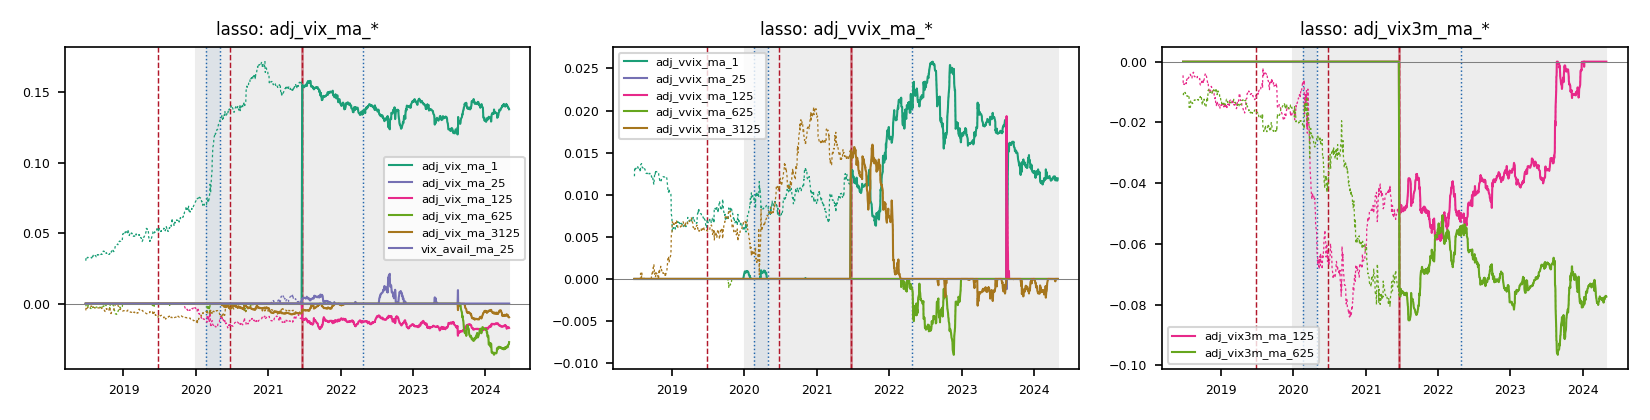
\includegraphics[width=\textwidth]{../results/model_diagnostics_1530/regimes_lasso_vix.png}
\caption{The lasso's standardized weights on the VIX-family columns (design column names; colour = lag as in Figure 1): solid = lasso of record, dashed = penalty held at 0.001 from the start. Thick red line = the lasso's penalty re-choice; other lines as in Figure 4. Only columns the lasso of record ever keeps are drawn.}
\end{figure}

\begin{table}[h]\centering\scriptsize
\caption{VIX-family columns in the lasso: refits (of 1,469) and deck days with a nonzero weight, share positive, mean standardized weight when nonzero, first nonzero refit, number of entries and exits; with the penalty held at 0.001: refits nonzero before 2021-06-21 (of 750) and the mean weight there.}
\resizebox{\textwidth}{!}{\begin{tabular}{lrrrrlrrr}\toprule
column & refits & deck days & positive & mean std.\ weight & first & entries/exits & held: refits before & held: mean \\\midrule
\texttt{adj\_vix\_ma\_1} & 719 & 636 & 100\% & +0.1388 & 2021-06-21 & 1 & 750 & +0.0923 \\
\texttt{adj\_vix\_ma\_25} & 215 & 174 & 100\% & +0.0052 & 2021-06-21 & 18 & 100 & +0.0030 \\
\texttt{adj\_vix\_ma\_125} & 719 & 636 & 0\% & -0.0143 & 2021-06-21 & 1 & 414 & -0.0109 \\
\texttt{adj\_vix\_ma\_625} & 170 & 169 & 0\% & -0.0245 & 2023-08-24 & 3 & 197 & -0.0022 \\
\texttt{adj\_vix\_ma\_3125} & 568 & 415 & 0\% & -0.0046 & 2020-05-07 & 15 & 741 & -0.0057 \\
\texttt{adj\_vvix\_ma\_1} & 767 & 664 & 100\% & +0.0155 & 2019-12-27 & 11 & 750 & +0.0092 \\
\texttt{adj\_vvix\_ma\_25} & 1 & 1 & 0\% & -0.0012 & 2023-08-16 & 2 & 0 & -- \\
\texttt{adj\_vvix\_ma\_125} & 9 & 9 & 100\% & +0.0089 & 2023-08-15 & 4 & 0 & -- \\
\texttt{adj\_vvix\_ma\_625} & 205 & 190 & 0\% & -0.0035 & 2022-03-02 & 6 & 15 & -0.0005 \\
\texttt{adj\_vvix\_ma\_3125} & 366 & 301 & 47\% & +0.0043 & 2021-06-21 & 32 & 698 & +0.0089 \\
\texttt{adj\_vix3m\_ma\_125} & 634 & 551 & 0\% & -0.0376 & 2021-06-21 & 6 & 750 & -0.0309 \\
\texttt{adj\_vix3m\_ma\_625} & 719 & 636 & 0\% & -0.0714 & 2021-06-21 & 1 & 750 & -0.0302 \\
\texttt{vix\_avail\_ma\_25} & 5 & 5 & 0\% & -0.0001 & 2022-08-10 & 4 & 0 & -- \\
\texttt{vvix\_avail\_ma\_1} & 0 & 0 & -- & -- & -- & 0 & 416 & +0.0061 \\
\bottomrule\end{tabular}}\end{table}

\enlargethispage{3\baselineskip}
\textbf{Reading.}
\begin{itemize}\itemsep1pt
\item \emph{The VIX enters at the penalty re-choice, not at an event.} Before 2021-06-21 no VIX-family column in the lasso of record exceeds 0.0076 in standardized weight. On 2021-06-21, when the penalty drops to 0.001, \texttt{adj\_vix\_ma\_1} enters and stays on all 719 later refits, always positive (mean +0.139), with the longer VIX3M means negative (\texttt{adj\_vix3m\_ma\_625} -0.071, \texttt{adj\_vix3m\_ma\_125} -0.038): the VIX's last bar against the 3-month index's longer averages.
\item \emph{The VIX was in the data before.} Held at 0.001 from the start, the lasso keeps \texttt{adj\_vix\_ma\_1} on 750 of the 750 earlier refits (mean +0.092) and \texttt{adj\_vix3m\_ma\_625} negative on 750, through COVID. The top-of-grid penalty kept the VIX out until 2021.
\item \emph{Entries and exits in between are small.} Of the 104 VIX-family entries and exits, 7 are at the penalty re-choice and 97 in the day-to-day path; after a day-to-day entry no weight exceeds 0.0177. None marks COVID or every-day expirations.
\item \emph{The lasso leans on the VIX more than the ridge.} Share of mean $|$SHAP$|$ on deck days: VIX 9.8\% and VIX3M 8.8\% (ridge 4.8\% and 5.1\%); realized variance 44.1\% (ridge 28.2\%).
\end{itemize}
Files: \texttt{experiments/model\_diagnostics\_1530\_regimes.py}; outputs \texttt{results/model\_diagnostics\_1530/regimes\_*}.

\end{document}
